\documentclass[aspectratio=169]{beamer}

% Shared Beamer settings for Elements of AIML lectures (UPES).
% Keep this file free of \documentclass to allow reuse via \input.

% Allow lecture sources to use shared theme/assets without copying them into each lecture folder.
% NOTE: These paths are relative to `Unit-xx/Lecture-yy/latex/` (and `Lab/Experiment-xx/latex/`).
\makeatletter
\def\input@path{{../../../_shared/}{../../../_shared/UPES-Beamer-Theme/}}
\makeatother

\usetheme{UPES}
\setbeamertemplate{navigation symbols}{}

\usepackage{amsmath}
\usepackage{amssymb}
\usepackage{booktabs}
\usepackage{graphicx}
\usepackage{hyperref}
\usepackage{xcolor}
\usepackage{listings}

% Code listings (general-purpose).
\lstset{
  basicstyle=\ttfamily\small,
  keywordstyle=\color{blue},
  commentstyle=\color{gray},
  stringstyle=\color{teal},
  showstringspaces=false,
  columns=fullflexible,
  breaklines=true
}

\usepackage{tikz}
\usetikzlibrary{arrows.meta,positioning,shapes.geometric,calc}

% Per-slide source line (references shown on the slide itself).
\newcommand{\slidesources}[1]{%
  \vfill
  {\tiny\color{gray}\raggedright\sloppy\parbox{\linewidth}{Sources: #1}\par}%
}

% Unit-wise source strings for this subject (used by slides/notes).
% Path is relative to the lecture `latex/` folder (the compilation CWD).
% Source strings for Elements of AIML (used by slides + notes).

\newcommand{\AIMLRepoURL}{https://github.com/tali7c/Elements-of-AIML}

\newcommand{\AIMLLabSources}{%
Provost and Fawcett, \textit{Data Science for Business}.;%
McKinney, \textit{Python for Data Analysis}.;%
WEKA Documentation (Waikato Environment for Knowledge Analysis), accessed 2026-02-28.;%
Matplotlib and Seaborn documentation, accessed 2026-02-28.%
}

\newcommand{\AIMLUnitISources}{%
Rich and Knight, \textit{Artificial Intelligence}, McGraw Hill, 2017.;%
Russell and Norvig, \textit{Artificial Intelligence: A Modern Approach} (4e), Ch. 1--2 (Introduction, Intelligent Agents).;%
Poole and Mackworth, \textit{Artificial Intelligence: Foundations of Computational Agents} (2e), selected sections.%
}

\newcommand{\AIMLUnitIISources}{%
Russell and Norvig, \textit{Artificial Intelligence: A Modern Approach} (4e), Ch. 7--9 (Logical Agents, First-Order Logic, Inference).;%
Huth and Ryan, \textit{Logic in Computer Science} (2e), selected sections on propositional and first-order logic.;%
Genesereth and Nilsson, \textit{Logical Foundations of Artificial Intelligence}, selected chapters.%
}

\newcommand{\AIMLUnitIIISources}{%
Mueller and Massaron, \textit{Machine Learning for Dummies}, For Dummies, 2016.;%
Mitchell, \textit{Machine Learning}, selected chapters on learning basics and evaluation.;%
Scikit-learn documentation, accessed 2026-02-28.%
}

\newcommand{\AIMLUnitIVSources}{%
Mueller and Massaron, \textit{Machine Learning for Dummies}, For Dummies, 2016.;%
James, Witten, Hastie, and Tibshirani, \textit{An Introduction to Statistical Learning} (2e), selected chapters.;%
Scikit-learn documentation, accessed 2026-02-28.%
}

\newcommand{\AIMLUnitVSources}{%
NIST, \textit{AI Risk Management Framework (AI RMF 1.0)}, 2023.;%
Barocas, Hardt, and Narayanan, \textit{Fairness and Machine Learning} (online book), selected sections.;%
Knaflic, \textit{Storytelling with Data}, selected chapters on communicating results.%
}



\title[Elements of AIML]{Elements of AIML}
\subtitle{Unit 03 -- Lecture 02: Train/Test/Validation Split \& Cross-Validation}
\author{Tofik Ali}
\institute{School of Computer Science, UPES Dehradun}
\date{\today}

\graphicspath{{../images/}{../../../_shared/}{../../../_shared/UPES-Beamer-Theme/}}

\begin{document}

\UPESCoverFrame
\setcounter{framenumber}{0}

\begin{frame}
  \titlepage
  \vspace{0.3em}
  \begin{center}
    \footnotesize Topic focus: \textbf{evaluation without fooling yourself} (splits, CV, leakage)\\[0.25em]
    \footnotesize Repository: \texttt{\AIMLRepoURL}
  \end{center}
  \slidesources{\AIMLUnitIIISources}
\end{frame}

\begin{frame}{Quick Links}
  \centering
  \hyperlink{sec:splits}{\beamerbutton{Splits}}\hspace{0.6em}
  \hyperlink{sec:cv}{\beamerbutton{Cross-Validation}}\hspace{0.6em}
  \hyperlink{sec:leak}{\beamerbutton{Leakage}}\hspace{0.6em}
  \hyperlink{sec:code}{\beamerbutton{Code}}\hspace{0.6em}
  \hyperlink{sec:summary}{\beamerbutton{Summary}}
\end{frame}

\begin{frame}{Agenda}
  \tableofcontents
\end{frame}

\section{Splits}
\label{sec:splits}

\begin{frame}{Learning Outcomes}
  By the end of this lecture, you should be able to:
  \begin{itemize}[<+->]
    \item Explain why we split data into train/validation/test sets.
    \item Describe what decisions are allowed using each split.
    \item Explain k-fold cross-validation and stratification.
    \item Identify common data leakage patterns and avoid them.
  \end{itemize}
\end{frame}

\begin{frame}{Abbreviations \& Symbols}
  \begin{itemize}[<+->]
    \item Train/Val/Test: training/validation/testing splits
    \item CV: cross-validation \hfill $k$: number of folds
    \item $\hat{y}$: predictions \hfill metric: accuracy/F1/RMSE, etc.
    \item Hyperparameter: setting chosen by us (e.g., depth, $C$, $\lambda$)
    \item Leakage: using information unavailable at prediction time
  \end{itemize}
\end{frame}

\begin{frame}{Why Split the Dataset?}
  \begin{itemize}[<+->]
    \item Goal: estimate performance on \textbf{unseen} data (generalization).
    \item If we evaluate on training data, we can be fooled by \textbf{overfitting}.
    \item Splits create a clean separation between learning and evaluation.
  \end{itemize}
\end{frame}

\begin{frame}{Train vs Validation vs Test}
  \begin{itemize}[<+->]
    \item \textbf{Train set}: fit model parameters.
    \item \textbf{Validation set}: choose model/hyperparameters (tuning).
    \item \textbf{Test set}: final unbiased evaluation (use once at the end).
  \end{itemize}
  \vspace{0.4em}
  Rule: do not repeatedly tune using the test set (it becomes a validation set).
\end{frame}

\begin{frame}{Split Diagram (Hold-out Evaluation)}
  \centering
  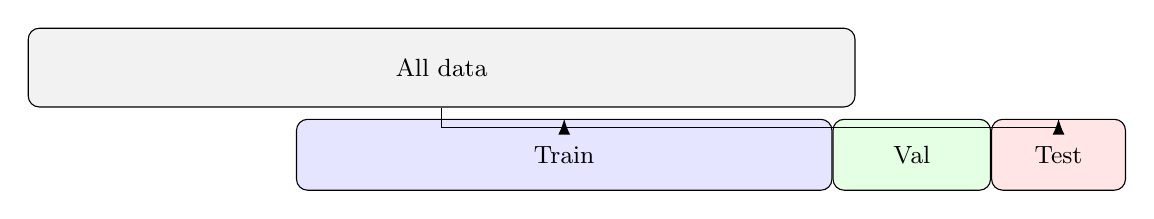
\begin{tikzpicture}[every node/.style={font=\small}]
    \node[draw, rounded corners, fill=gray!10, minimum width=10.5cm, minimum height=1.0cm] (all) {All data};
    \node[draw, rounded corners, fill=blue!10, below=0.6cm of all, minimum width=6.8cm, minimum height=0.9cm, anchor=west, xshift=-1.85cm] (train) {Train};
    \node[draw, rounded corners, fill=green!10, right=0cm of train, minimum width=2.0cm, minimum height=0.9cm] (val) {Val};
    \node[draw, rounded corners, fill=red!10, right=0cm of val, minimum width=1.7cm, minimum height=0.9cm] (test) {Test};
    \draw[-{Latex[length=2mm]}] (all.south) -- ++(0,-0.25) -| (train.north);
    \draw[-{Latex[length=2mm]}] (all.south) -- ++(0,-0.25) -| (test.north);
  \end{tikzpicture}
  \vspace{0.4em}
  \small Tune on \textbf{Val} (or CV), report final score on \textbf{Test} once.
\end{frame}

\section{Cross-validation}
\label{sec:cv}

\begin{frame}{Cross-Validation (k-fold)}
  \begin{itemize}[<+->]
    \item Split training data into $k$ folds.
    \item Train on $k-1$ folds, validate on the remaining fold.
    \item Repeat for all folds; average performance.
  \end{itemize}
  \vspace{0.4em}
  Benefits: more stable estimate, better use of limited data.
\end{frame}

\begin{frame}{k-Fold Intuition (What happens each round?)}
  \centering
  \begin{tabular}{l}
    \toprule
    Round 1: \fbox{Val} | Train | Train | Train | Train \\
    Round 2: Train | \fbox{Val} | Train | Train | Train \\
    Round 3: Train | Train | \fbox{Val} | Train | Train \\
    \dots \\
    \bottomrule
  \end{tabular}
  \vspace{0.4em}
  \small Average the validation metric over rounds; then retrain on all training data with chosen settings.
\end{frame}

\begin{frame}{Stratification (Classification)}
  For classification, ensure each fold keeps class proportions similar to the full dataset.
  \vspace{0.4em}
  \begin{exampleblock}{Why it matters}
    If a fold has almost no positive examples, metrics like recall become meaningless.
  \end{exampleblock}
\end{frame}

\section{Leakage}
\label{sec:leak}

\begin{frame}{Data Leakage: A Silent Killer}
  Leakage = using information that would not be available at prediction time.
  \vspace{0.4em}
  \begin{itemize}[<+->]
    \item Using post-event fields (e.g., ``approved\_date'' to predict approval)
    \item Preprocessing using the full dataset before splitting (e.g., scaling using all data)
    \item Duplicates across train and test (near-identical samples)
  \end{itemize}
\end{frame}

\begin{frame}{Leakage Prevention Rules (Checklist)}
  \begin{itemize}[<+->]
    \item Split first, then fit preprocessing on \textbf{train only}
    \item Do feature selection inside CV (not before)
    \item Keep duplicates/groups in a single split (GroupKFold when needed)
    \item For time series, split by time (no future $\rightarrow$ past)
  \end{itemize}
\end{frame}

\section{Code}
\label{sec:code}

\begin{frame}[fragile]{Minimal Code Pattern (scikit-learn)}
  \begin{lstlisting}[language=Python]
from sklearn.model_selection import train_test_split

X_train, X_test, y_train, y_test = train_test_split(
    X, y, test_size=0.2, random_state=42, stratify=y
)
  \end{lstlisting}
  \vspace{0.3em}
  Always fit preprocessing \emph{only on training data}, then apply to validation/test.
\end{frame}

\begin{frame}[fragile]{Leakage-Safe Pattern (Pipeline)}
  \begin{lstlisting}[language=Python]
from sklearn.pipeline import Pipeline
from sklearn.preprocessing import StandardScaler
from sklearn.linear_model import LogisticRegression

pipe = Pipeline([
    ("scaler", StandardScaler()),
    ("clf", LogisticRegression())
])
  \end{lstlisting}
  \vspace{0.3em}
  With CV, the scaler is fit \textbf{inside each fold} (safer).
\end{frame}

\begin{frame}[fragile]{k-Fold Cross-Validation (sketch)}
  \begin{lstlisting}[language=Python]
from sklearn.model_selection import StratifiedKFold

cv = StratifiedKFold(n_splits=5, shuffle=True, random_state=42)
for train_idx, val_idx in cv.split(X, y):
    X_tr, X_val = X[train_idx], X[val_idx]
    y_tr, y_val = y[train_idx], y[val_idx]
  \end{lstlisting}
\end{frame}

\section{Summary}
\label{sec:summary}

\begin{frame}{Summary}
  \begin{itemize}
    \item Splits protect us from overfitting and give honest evaluation.
    \item Validation is for tuning; test is for the final report.
    \item Cross-validation improves stability when data is limited.
    \item Leakage can make results look great but fail in production.
  \end{itemize}
  \slidesources{\AIMLUnitIIISources}
\end{frame}

\begin{frame}{Exit Questions}
  \begin{enumerate}
    \item Why should the test set be used only once at the end?
    \item What is cross-validation and when do we use it?
    \item Give two examples of data leakage.
    \item What does stratification mean and why is it used?
  \end{enumerate}
\end{frame}

\end{document}
